\documentclass[12pt]{article}
\usepackage{graphicx}
\usepackage{ltablex}

\title{Dungeon Crawler CO3 Computer Science Programming Project}
\author{William Riddell}

\begin{document}
	\pagenumbering{gobble}
	\maketitle
	
	\newpage
	\pagenumbering{arabic}
	\tableofcontents
	
\section{Analysis of the problem}
	
	\section{Problem Identification}
	
		\subsection{What will be developed}
I will be hoping to develop a Medieval dungeon crawler game in C\#, which is using the Visual Studio 2017 IDE. The game will allow the user to move their character around a randomly generated dungeon. This dungeon will look like a maze, with dead ends and loops, where the player will encounter monsters, trap rooms and treasure rooms. This is where the player will grow in power, by upgrading their statistics; like strength, carry weight, stamina etc. As the player moves through the dungeon the enemies will get stronger as the player levels up, until they encounter the Boss Room. This is where the character has to beat the Boss in a final battle to win the game. If the player dies within the dungeon then they lose, and they then must create a new starting character and begin all over again, growing stronger along the way to try to defeat the final Boss again.

The Setting for the game will be in a dark dungeon, with set back grounds which indicate where the dungeon will lead for the character, be it if there is a left turn, right turn, both, if it continues etc. I could have doors drawn into the background which could indicate the different rooms. Parts of the dungeon which haven't been visited yet will be hidden from the player, so they don't know what is inside the room. This means that they can move into a trap room at any time. Once the player is in a room though, they can “run” to the last tile they were at. This means that they have the option to not fight the monster, and instead take a different route. 

There will be a small menu in the very middle bottom which will give the player all the options which are open to them, be it to move in a certain direction, and then to the side of their options, but still in the same box there will be the description of the current room. The menu will change when the player encounters an . The menu will show more options, these options are;monster change which weapon they want to fight with. weapon, it changes the icon displayed next to the character menu (Which will be talked about later) showing how much base damage and the multipliers the current weapon has.The menu will give a description of what is contained in the current tile, and if a monster is in the tile, a description of the monster. This menu will allow the player to change their equipped weapon. 

There will also be text which appears. This text describes the damage dealt or taken. This text will be located just right of the very middle of the screen and will keep the player up to date on what is happening in the battle, allowing them to make better decisions when playing through the game. and will be there to tell the user what is happening in the current fight so they can make the correct decisions. It is also there to make sure the user does not miss any important information which may lead to them losing the game. 

There will be a small screen just to the left of the bottom menu, which will show the current statistics on the character. This will show the health of the player, their carry weight and then their currently equipped weapon. This will also show the currently equipped armor as well, showing what the player has a resistance too, and then the amount of damage it will deal to each type of monster.  

To the right of the bottom menu, there will be the inventory, this will include, for example provision, gold and other treasures, as well as items like a sword and armor, it will also have items like torches. Extending this there will be a finite number of spaces in the inventory, this limits the space which the player has, meaning that they have to prioritise what they want to carry.

There will be a mini-map in the top right which will give a localised view of the area surrounding the player, showing only where they have been, and if they click this it will show a full map, meaning they can plan their route out, or explore areas. 

If the player presses a certain button (Escape for example) it will open a main menu, pausing the game in the background and allowing the player to save, overwrite saves or quitting. Having this save feature will allow people to pick it up, and to then come back to it as the game, on the harder difficulties and on a bigger map will last for quite some time, meaning this would be a crucial feature.

	\section{Computational Methods}

		\subsection{Thinking Abstractly and Visually}
I need to begin to think Abstractly and Visually, this is because it would be impossible to accurately simulate everything which would happen in the dungeon, and would also be impossible to code, this is because of my own limitations and ideas. This means that some ideas will be lost for a more simple reconstruction which achieves the same effect. This could be for example when battling monsters, the monsters will have a single simple attack, and then multipliers which will be added to the attack. This means that it simplifies the idea that if the monster was real then it would instead have an array of different attack styles which will all do different “damages”. Another example is that different attack styles would do different amounts of damage against different armor. This could be simplified with armor levels, as light armor like leather or chain-mail would absorb less damage and would therefore have a lower armor level. This is a abstract of real life as if you take light armor it allows the person to have more maneuverability, but at the same it would take less damage against certain weapons. 

There are certain aspects of real life which I was not sure if I was going to include or not, this were aspects of life like eating and drinking. I was also thinking about including the idea that when you are damaged you deal less damage, as this would be similar to real life. After talking to my Stakeholders I have came to the final conclusion that eating and drinking would take too much effort to keep track of, and would take away from the core idea of the game. They would also think that the idea about decreasing the amount of damage that you do was a good idea at first, and then later Jimbo came back and said that it wouldn't actually be a good idea, so I don't think I will be including any of these aspects as it would be too close to real life and would take away from the main idea of the game, it would also feel unfair for the user to die in battles because of a strong hit by the enemy. 

	
		\subsection{Thinking Ahead}
	
When coding the dungeon crawler I need to look at the inputs which are needed for the game. I think that I would need the mouse for the user to select what options they want and what action they would want the character to do. This would be the first input. I would also need the keyboard as this would allow the user to input the name and other information about their character. After this I would mainly use the mouse, and the keyboard would become unnecessary. 

When coding my game I will need to code in error handling, this is when the player enters the wrong data type for example, and without the error handling the whole code will break, as there wouldn't be the expected data type, and would therefore go wrong when I try to work out values. Null values may also break my code, and I need to catch any errors when they appear.   

		\subsection{Thinking Procedurally and Decomposistionally}
	
My problem can be broken down into sections. I can separate the windows into a main menu, this would allow the player to select what they would want to do, this could be to open the options, to exit or to load up a old save or to make a new one. Each of these options will lead on to the next window. Each window will contain its own menus, only building what it needs and when it needs it. Having the forms like this means that the code will be much faster as it will be more optimised as it will only need to load up the menus which it needs. When the game loads the game make a new maze, this maze will be built from Tiles, and these tiles will contain either a monster or a room. There will be a tile class which means I can have a maze of any size as I can just make more tile objects. When I populate the maze with rooms, some of the tiles will be assigned a room, if it is not assigned a room, the tile will have the room value of null and will not contain a room. The same method will be applied to the monsters, as this will allow a even spread of monsters to be applied to the maze of any size. 

As the player moves through the maze he will pick up items from the ground, this will be stored in their inventory. This will be a parent class, and then there will be a class for Gold, armor and then other misc items which for example could be potions. Having inheritance means that I only need to code certain aspects of each item once, as they all share the some of the same properties, such as being a item which can be stored in the players inventory.  

		\subsection{Thinking Logically}

When thinking logically, it concerns the idea of thinking with iterations and selection. There will be multiple loops in my code. On a larger scale the game doesn't have too much iteration, the game will have replayability though, and the user will have to make decisions, but the computer doesn't have to make many decisions itself, instead it just reacts to what the user chooses to do in simple ways.

When looking at the code there is a lot of For loops, this is classed under iteration. We can see that it is used when moving through the 2D arrays of tiles. When deciding what to do the computer uses If statements, this is called selection, and there will be multiple of if statements throughout my code, for example when the user has found a treasure room, the computer needs to send back the correct items contained in the room.


		\subsection{Thinking Concurrently}

In my game there isn't code which is called at the same time. Within my game everything is executed in steps, which is dependent on what the user chooses to do. 

Even when creating the maze there isn't any code which is executed at the same time as when the grid is created everything which is placed on to of it (The Monsters and the rooms) are all placed individually, I have executed my code this way to make sure that there isn't a monster placed over a monster etc. I could have 2 threads placing monsters throughout the maze if it is large enough, but at the current time there doesn't need to be another thread, so I will code this in at a later date if I have the time. 

	
	\section{Stake Holders}
	
	\section{Researching the Proposed Solution}
	
Information about my Stakeholders
My Stakeholders are Jimbo Giling, and Peter Cunningham. I think these two people will be suitable for my game as they both bring different angles to my project, and will input different views, ideas and solutions which appear. I know these people personally, and can easily contact them, this will allow me to get a fast response to my questions even in time outside college. Having this fast response means that I can tailor my game to fit them as they are in the target audience quickly and efficiently. 

I asked Jimbo to be my stakeholder because he will bring ideas for the enemies which the player will be encountering throughout the game. He has played many fantasy games which will give him a wide range of knowledge in enemies and encounters which I can code into my game. This will keep the game interesting even when the player is on a larger map. 

Peter is more interested with the design of the character. He can bring armor, weapon and other item ideas. This could be the items which they are picking up, or the apparel which they wear as well as the apparel on the monsters. Peter can also help me with the HUD (Heads up Display) which could also be called the user interface, the HUD is a crucial part of the game, as this is what they will be interacting with, so a HUD which is simple to use and aesthetically pleasing would be crucial. 

I think Jimbo and Peter alike have felt a dissatisfaction in the current release of RPG games and how alike the game-play is in all of them. This is why they are both looking forward to my randomly generated levels and interesting encounters. Peter has also found a lack of a challenge in current games, and therefore means that he loses interest in the games which he plays, so having a level system would suit him massively. 

Jimbo took GCSE art, this will allow me to ask him about my art work, and will take ideas which he produces, making sure that the HUD and the monster design is to a certain quality. Peter plays a lot of single player games, this forces me to keep the game to a high quality so it keeps him interested.

	
		\subsection{Similar Solutions}
	
			\subsubsection{Random Generation}
I looked at a game called “Rebuild”. In this game you are placed in a post apocalyptic world surrounded by zombies. The goal is to grow your base and survive until you reach a win condition. Every time you load into a new City the terrain around you will change, for example in this game I have a Mall next to my base:

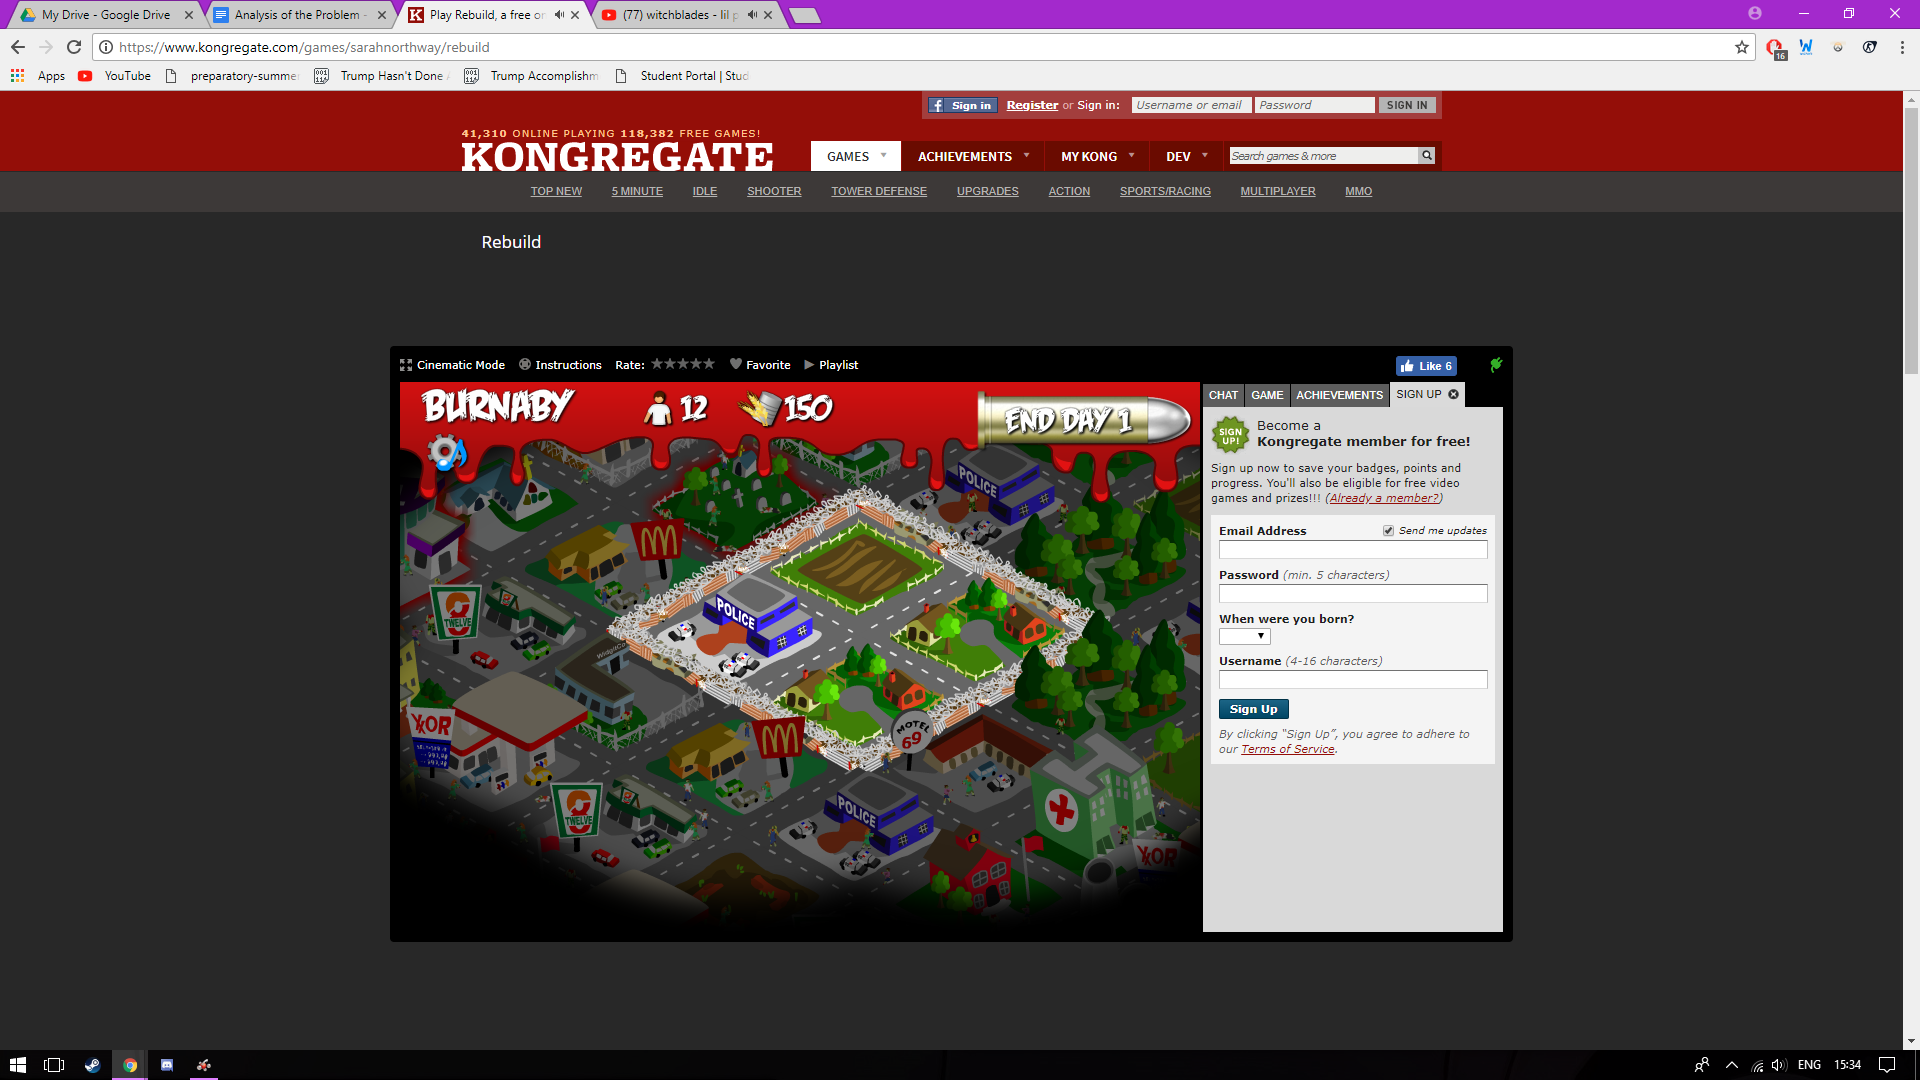
\includegraphics[width = 0.6\textwidth]{Rebuild_Image}

In this game there are constants, you are given 12 people and 150 food to start with (This is in the top bar in each image). This is a good idea as this means when you start a new game you always know that you will have a strong start, and then from them you  
	
			\subsubsection{Ramping Difficulty}
			
Furthermore in Rebuild, the zombie attacks on you city ramp over time, meaning it is always getting harder and more challenging. I would like to include this in my own project so the game doesn't get too easy in the late game, and also meaning the final boss will be around the same difficulty no matter when you face it in the game. I can either do this as time goes on, which is how this game works, or instead the average XP of the players characters. This will be standard for all difficulties, so when you select easy, the game will be easy thought out, or when you select hard, it is still hard until the very end. 
	
			\subsubsection{Appearance and Audio}
			
I much prefer having my game first person, this will increase the connection the player has to the characters, as well as increasing immersion. Even though the graphics are not realistic, I would like the audio to be convincing. So I will be looking for copyright free audio samples which I could use on my game. I wouldn’t be able to achieve graphics like this so I would like to do basic pixel art, as this is more accessible for me. This will allow me to use skills which I have learned in GCSE art, and also to ask Jimbo, my stakeholder with advice for this as he also took GCSE art. 

I have found a game called the Legend of Grimrock. This is what it looks like:

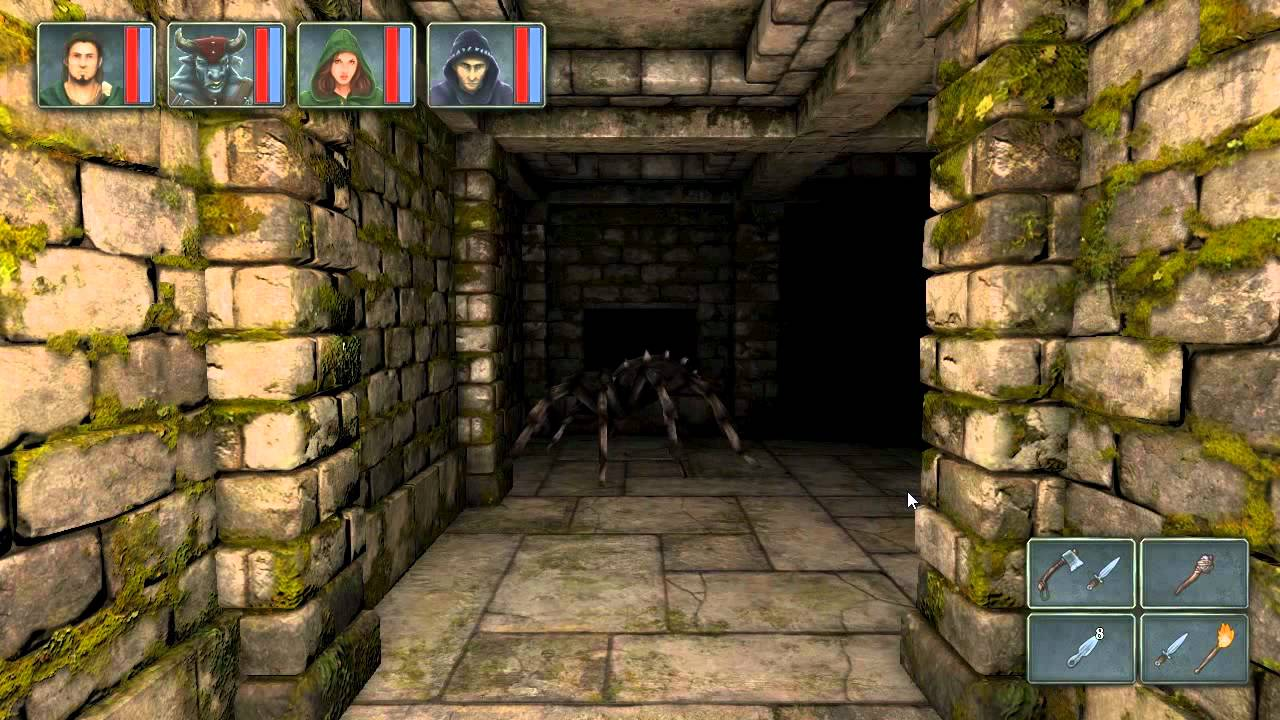
\includegraphics[width = 0.6\textwidth]{Grimlock_Image}

As you can see, it has items in the bottom right, and characters in the top left. This is somewhat what I would like my game to looks like referencing the HUD, but the background is exactly what I would like it to look like, although the graphics would be in a pixel art style, and will be 2D. I would like enemies to appear in front of the player when the player enters that monsters square. I don't know whether I will indicate what is in the next tile at this point in time. Furthermore I would like the enemies to have an indicator for the Health and other statistics, to give the character information about what they are facing. This is contained in to top left with each Character, but I will only have one character which the player will play as. This means I think I will have a separate menu section for the health and statistics which will be in the bottom left. 

After talking to my stakeholders I should not indicate what is in the next rooms, but instead indicate where they can next go. This will keep the idea that everything is random until discovered and entered.

The inventory on the right will be exactly like that, but with an increased number of slots which is dictated by the characters carry weight, and inside the slots the item which they are carrying.

	
			\subsubsection{Combat}

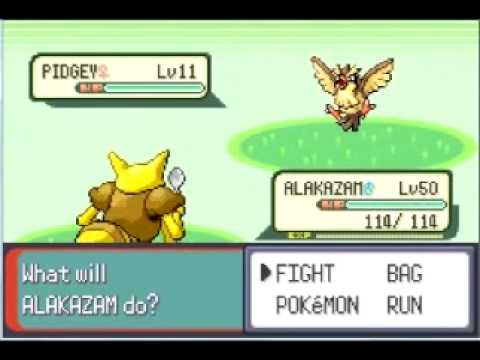
\includegraphics[width = 0.6\textwidth]{Pokemon_Image}

The game above is Pokemon, I will be taking the combat system from this game. As you can see there is the Players Pokemon in the foreground and then the enemy’s Pokemon in the background, and to the side of each Pokemon there are statistics which are displayed to the player. This tells the name of the two Pokemon battling, the level of the two Pokemon and the health of the Pokemon. Furthermore there is a menu at the bottom of the screen which displays text to the player and then options which they can select. 

When you enter a battle with an enemy you decide what to do on your first turn. This could be to “Fight” and then you can select the attack which you will use. You could use something from you bag, this could be to increase the HP of the Pokemon on the field. If your current Pokemon is low, “KO” (This means it can’t be used) or too weak you can swap it out for another Pokemon. Finally, if you are going to lose this battle you can run, allowing you to safely move on. Pokemons combat is turn based.

I would like to implement all of these features into my game. For the “Fight” button, you could select the style of attack to use, for example you could “Lunge” this, for example could be a high damage, but low accuracy attack, compared to a “Stab” where it could be very accurate, but low damage. I could further this with multipliers, for example a “Slash” attack is weaker on armored opponents, yet stronger on less armored enemies. This can further develop the depth of the game, as as you move on and spot the boss,you can prepare your character to deal with that Boss type, which is dictated from the multipliers. For example there could be an Undead Boss, which means you should try to find weapons and armor which is more adapt to dealing with undead characters, which could be a fire based attack, or the slash attack we talked about earlier.

The player should have an option to use their turn by selecting an item their inventory. This could be switching weapons, or using some provisions to heal up their character if they are low on HP. Finally, you should be able to run away from the enemy, this means that you move to the room you were last in. This will be used to take a different path way if there is a strong monster in the way.
	
		\subsection{Stakeholder Questionnaire}

This is the Questionnaire which I will be sending to my stakeholders. The answers to the questionnaire will be stated below.

\begin{enumerate}
	\item{Would you like random monsters to be generated through out the grid?}
		\begin{enumerate}
		\item Yes
			\begin{enumerate}
				\item If so, what statistics should be randomised?
				\item Should I make every enemy be around the same difficulty?
				\item Should I have multipliers? For example, this monster has a specific weakness to fire.
				\item Other Ideas
			\end{enumerate}
		\item No
			\begin{enumerate}
				\item How many monsters should I set?
			\end{enumerate}
		\end{enumerate}

			
	\item{Should I limit my inventory?}
		\begin{enumerate}
		\item Yes
			\begin{enumerate}
				\item The carry weight integer should be the number of items a single character should hold
				\item Some items should not be carried, for example arrows. 
			\end{enumerate}
		\item No
		\end{enumerate}
			
	\item{Should I add a scoring system?}
		\begin{enumerate}
		\item Yes
		\item No
		\end{enumerate}
			
	\item{Should I add a constant music, maybe ambiance?}
		\begin{enumerate}
		\item Yes
		\item No
		\end{enumerate}
				
	\item{Should I add audio cues, for example when you reach a treasure room, there is a small jingle which plays?}
		\begin{enumerate}
		\item Yes
		\item No
		\end{enumerate}
			
	\item{Should all the dungeons be the same, or should I change to a different background, for example it could be inside a pyramid?}
		\begin{enumerate}
		\item Yes
		\item No
		\end{enumerate}

	\item{Should the user be able to see all of the map?}
		\begin{enumerate}
		\item Yes
		\item No
			\begin{enumerate}
				\item How much should I limit it by? Or should I only allow the player to view the tiles which trhey have been on?
			\end{enumerate}
		\end{enumerate}

			
	\item{Should I have a constant mini-map in the main form, or should I have a map form which they can always keep open?}
		\begin{enumerate}
		\item You should have it in the Mini Map style
		\item It should be contained in a separate form
		\end{enumerate}
			
	\item{Please enter further ideas on the game.}
\end{enumerate}	



			\subsubsection{Stakeholders Response}


I have kept this questionnaire short, and specific. I believe this will be better as I already have a good view of what I would like the game to look like. Although on some areas, im not too sure what to do and this is why I have asked my stakeholders. This will allow me to clarify what to do and how to attack these problems, as well as giving me new ideas to develop and move into the game. I can also ask my stakeholders throughout my project, as they are easy to contact them to get a quick answer.




\centerline{Peters response:}

\begin{enumerate}
	\item{Yes, I think you should have range where the monsters health, attack damage etc should be. \\}
	\em{This response was originally in line with my own opinions, as this will keep the mystery when moving into another tile, and facing a random boss.}
	
	\item{Yes, I think the inventory should be a visual grid, here there is a limited amount of squares. \\}
	\em{Peter gave the example of the game Runescape, the inventory looked like this:\\}
	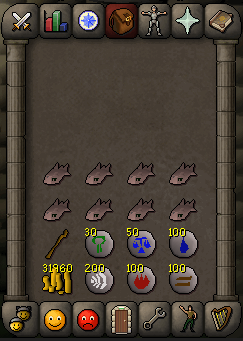
\includegraphics[width = 0.4\textwidth]{RuneScape_Image}
	\\
	\em{This is the inventory which I will be going with, but I will have the spaces grow with the characters carry weight.}
	
	\item{I think there should not be a underlying score, and the win condition should only be if you have killed the final boss. I also think when you die, you die.\\}
	\em{I don't think a underlying score would be good either, as this wouldn't be fair as longer games would yield a higher score, and would therefore be unfair.}
	
	\item{Yes, I think there should be music and ambiance\\}	
	\em{Making and finding music is hard, but I think I will be able to find some as I really want to have music in my game, as all of us want music in the game.}
	
	\item{Yes\\}
	\em{I want to make my own jingle here, as I want it to be specific to the game.}
	
	\item{There should be a variety of different biomes, for examples barbarian, Arabic / Indian as well as the Egyptian one.\\}
	\em{I really like the idea of the Egyptian and the Indian biomes, these will both be contained in the final game if I have time.}
	
	\item{No, when the player first spawns there should be a certain amount of tiles which are allowed to see, and then the rest should only become visible when the player visits them \\}
	\em{This will allow the user to get a strong start, and not get killed at the beginning of the game. A problem with this is that you may be spawned next to a treasure room, and they won't have the luck of finding one, as it would be displayed that they were spawned next to it.}
	
	\item{There should be a small mini map, and the a big main form. The main form will show you the whole size of the map, and the mini-map only a small amount of the map \\}
	\em{I like this idea a lot but I don't see the need of it if you can just have the main map form open in another window.}
	
	\item{I think there should be a Shop Room, this is where the player can sell his Gold which he has earn't from killing monsters. \\}
	\em{This is a very good idea and I want to contain it in the final version of the game as it encouraged the player to tailor their character to the final Boss.}
\end{enumerate}





\centerline{Jimbo's Response:}

\begin{enumerate}
	\item{No, there should be set monsters, as when you encounter them, you know if you can take them on or not, and if you can't then you can run away. \\}
	\em{This makes sense as this allows you to predict what you are going up against which allows you to calculate if you can take the battle or not. This will allow consistency for the player.}
	
	\item{No, you should be able to carry as much as you like, but there should be a limit, and when you reach that limit you have a de-buff, this is when you do less attack damage for example \\}
	\em{This is unlike Peters idea, what Jimbo is saying is that you can carry as much as you like, but the character has a certain value which, when exceeded your character has a multiplier to them, maybe making them weaker, or to tier easier in battle. I think I will still choose Peters idea, as this seems to make the most sense and is the closest to reality.}
	
	\item{Yes, this should count monsters killed, your characters level, the amount of Gold you have carried etc. But defeating the final Boss should be the only win condition. \\}
	\em{I disagree with this, as if you make a scoreboard, the person with the biggest maze can get a infinitely big score as the maze could be infinitely big.}
	
	\item{Yes, I think there should be both \\}
	\em{I think Jimbo wants a constant ambient sound in the background, this will add immersion to the game, but I think that making the ambiance would be too hard, and therefore I am going to try and find a copyright free ambient track.}
	
	\item{Yes, there should be a jingle for finding treasure, and killing the Boss \\}
	\em{I think this would be a nice idea as well, so I am going to try to contain some small jingles in my game, although I will try to make my own.}
	
	\item{Yes, There should be one set in Hell, under water etc, I also like the Pyramid idea a lot. \\}
	\em{It is good that we all like the pyramid idea, and the Hell and Underwater ideas would be interesting to make. Hopefully Jimbo could help me create the backgrounds.}
	
	\item{No, only tiles which the player has visited should be visible on the mini-map \\}
	\em{I agree with this point as it means that the player has to travel to the surrounding tiles, making the boss room a surprise, and also the trap rooms hidden.}
	
	\item{I think it should only be in a separate form \\}
	\em{This would be better for the user as it allows the to have it open on a different screen, or to have it constantly open in another window. This keeps the main form from being cluttered and will allow me to fit everything in with room to see the current tile.}
	
	\item{There should be battle pets to help you along the way, you should be able to carry gear, rings etc which all buff you, for example make you deal more damage. \\}
	\em{I never through about pets, this is a good idea but will be hard to code, so I think I will add it in later iterations. Other gear would be fairly easy to add but I also think I will add it in later iterations as it isn't needed.}
\end{enumerate}
			
		\subsection{Explaining the Solution}

“So what will the main menu look like?”
“I would like my main menu to be a full screen application, with 4 options. The first option is to make a new save, the second one is to load a save, the 3rd one brings up options and then the 4th option is to quit.”

“So what will happen when you select to make a new save?”
“When you make a new save, it will change the screen to another full screen form, which will allow you to select what statistics you want for your character, the size of the grid and also the difficulty.”

“And then what will happen if you select Load a save?”
“When you load a save, you will be asked to give a path to a file. This path will be given to you when you last saved the game, after this is would of then loaded you into the last tile which you were on”

“So what is a Tile?”
“The map is separated into Tiles, and in each tile is a area, or room which may contain an event, such as the Boss room, or having a monster inside of it etc. Some events may be good, like a treasure room, or bad like a trap room. This will be indicated on the map when it is opened.”

“What sort of monsters will there be? And what sort of Trap Rooms will there be?”
“Each monster, trap room, treasure room etc will all be randomised, although, I do want the randomised values to be in a bracket, so the player wont be facing any super hard or super easy monsters, or finding a treasure room, and getting nothing from it. The monsters will be from a set”

“So What will the actual game look like, once the player has loaded up their game?”
“I want my game to be in full screen, with buttons in the top right, which open the menu, and in the top left to open the map form. I also want there to be, in the bottom left, a image which displays what the current characters health is. I also want any buffs which he is given from the item which he is holding contained in this picture. To the right of the character window, in the middle of the screen, but still on the bottom of the screen, will be the main bar, this will contain the current options for the player, and also any information which they are given. To the right of this will be the inventory, which will contain all the items in a list form, and also indicating when the player is over encumbered, which will then cause de buffs to appear in the character window. In the main window, which will take up the rest of the screen will be the background, which is dictated by the tile type, and anything extra which is contained in the tile, like a chest or a monster.”

“What is the recommended audience?”
“I want my audience to be young adults, so around 17 to 18. This is because the game will be quite challenging and will also take up a lot of time. It could though appeal to a younger audience, as the game will include a setting to make the monsters easier. This is why I have chosen you three as the stakeholders, as you are all inside of my target audience age bracket.”

		
		\subsection{Limitations}

I think my limitations are the graphical side of the project, as this will be incredibly time consuming, and will also mean that I have to learn how to draw pixel art. Another problem will be the audio, as I have no idea where to get the samples, or how to make them, so that will also be a limitation of the project as both of my stakeholders have agreed that there should be music. I think that I will try to get a copyright free ambiance which I can use for the background, and then make my own jingle as a audio cue.

A coding limitation would be the user interface of the solution, with the menus, and the buttons and drawing the character and the inventory windows in the main game screen and achieving a professional look will be a challenge. I think getting the exact look that I want would be a struggle, but I think I could get a GUI which would be usable working.

Jimbo gave and idea for magic and battle pets, but at this point in time I don’t think that that would be feasible with the limited time of the project.

	
	\section{The Proposed Solution}

		\subsection{Requirements for the Solution}
	
\begin{tabularx}{\linewidth}{XXX}
Requirement No:         & Requirement                                                                                        & Justification                                                                                                                                                                                                                                      \\
For The Maze:           &                                                                                                    &                                                                                                                                                                                                                                                    \\
                        & To get the maze to be randomised, without any glitches or dead ends                                & This will allow a interesting game, every game. It allows the player to think about pathways, and to decide what monster to kill if there are multiple blocking their way.  
                        \\ 
                        \\                                                                      
                        & The Maze needs to be as big as the player wants it to                                              & This allows the game to take as much time as the player wants, meaning that                                                                                                                                                                       
                        \\
                         \\
                        & There should be monsters randomly scattered across the map                                         & This will allow the player to move around the map without knowing what is next                                                                                                                                                                    
                        \\
		     \\
                        & Each monster needs to be chosen from the list of monsters                                          & This will allow the player to remember what monsters there, but also for it to be less repetitive                                                                                                                                                  		     \\
                        \\
                        & The Boss room should be randomly placed                                                            & This will mean that the user can with the game.                                                                                                                                                                                                   \\ \\
                        & The maze shouldn't have any tiles which you can't visit                                            & This allows the user to fully explore the grid, and allow them                                                                                                                                                                                     \\
For the Main Game Form: &                                                                                                    &                                                                                                                                                                                                                                                    \\
                        & The window needs to take up the whole screen                                                       & This means that the player has a more immersive experience, where everything is more ordered as it branches from this one main window                                                                                                             \\ \\
                        & There should be a bottom bar, where the options and description is displayed                       & This will allow the player to select their options, it also allows them to get information for the tile which they are in This will allow the player to select their options, it also allows them to get information for the tile which they are in \\\\
                        & The options button should be functional and opens another form over the main form                & This will allow the user to exit the game, or save at any point                                                                                                                                                                                    \\\\
                        & There needs to be a menu which displays the current characters stats, like health and carry weight & This will allow the user to judge whether they can take the next fight                                                                                                                                                                             \\\\
                        & The map needs to be displayed in a different form when the user clicks the map button              & This will allow the user to see the map, allowing them to choose their path accordingly                                                                                                                                                            \\\\
                        & There should be an inventory window in the bottom right                                            & This will show the player what the have in their inventory, showing what items they have and how many they have of each item                                                                                                                       \\\\
Monster:                &                                                                                                    &                                                                                                                                                                                                                                                    \\\\
                        & Each monster needs to be from the class monsters, meaning its attacks and statistics are set.      & This will allow the user to predict if they can take the fight, and know what they are going to fight.                                                                                                                                             \\\\
                        & The monster needs to be draw to the form                                                           & This will allow the user to see the monster, allowing them to quickly recognize their enemy.                                                                                                                                                       \\\\
                        & The form’s options needs to change so he player can decide what to do                              & This will show the options to the user, allowing them to select what they want to do                                                                                                                                                               \\\\
                        & The monster inflicts damage and can take damage                                                    & This allows for combat which means the user can pass through the tile to the next area.                                                                                                                                                            \\\\
For the Character       &                                                                                                    &                                                                                                                                                                                                                                                    \\\\
                        & The statistics need to be shown correctly, and the be edited / modified correctly.                 & This will allow the user to see what their health and other statistics are, meaning that they can make educated decisions                                                                                                                          \\\\
                        & The character needs to have their modifiers displayed to the user                                  & This will allow the user to see what each item does, and the effect it has on them. This will allow them to choose what they want to equip                                                                                                        \\\\
Items                   &                                                                                                    &                                                                                                                                                                                                                                                    \\\\
                        & The items need to be correctly rendered in the inventory                                           & This will allow the user to see what they have, and if it is in use or not                                                                                                                                                                         \\\\
                        & The Items need to stack                                                                            & This will allow the user to store a lot of one item without filling up their inventory.                                                                                                                                                           
\end{tabularx}
		
		
		
		
		
		\subsection{Hardware and Software Configurations}
		

\begin{tabularx}{\linewidth}{XX}
CPU              & You will need a 2 Ghz or faster processor       \\\\
Memory           & You will need at least 4GB of RAM               \\\\
Storage          & You will need at least 2GB of storage           \\\\
Graphics Card    & You will need a DirectX Compatible 9 Card       \\\\
Operating System & You will need to run a Windows Operating system
\end{tabularx}



%%%%%%%%%%% 		END OF ANALYSIS OF THE SOLUTION 		%%%%%%%%%%%


\section{Iteration 1}

I started my development by asking my stakeholders what would they want to be implemented first, they said that I should work on generating the maze, and then placing the player inside of that maze, allowing them to move around it. I think i will further this idea by implementing monsters and the different types of rooms. This will lack the ability to allow the player to enter combat with the enemies, and the effects of the rooms would be into play, but the player can freely move around the maze. I think I will leave making the stats for the player until Iteration 2, and from there I can then develop out the combat as well. 


\begin{tabularx}{\linewidth}{XX}
Requirement                                                                                   & Time Cost \\ \\
To get the maze to be randomised, without any glitches or dead ends                           & 3 Hours   \\ \\
The Maze needs to be as big as the player wants it to                                         & 1 Hours   \\ \\
There should be monsters randomly scattered across the map                                    & 2 Hours   \\ \\
The player should be able to move around the grid one space at a time obeying the grids walls & 2 hours  
\end{tabularx}

The First 3 requirements are all about the maze generation. This will take just over a week to code, as the total approximate time which it will take is 5.5 Hours, which is 1.5 Hours over my allocated time per week. Regardless of it being over the time I have set aside for my project I should still be able to get this done. 

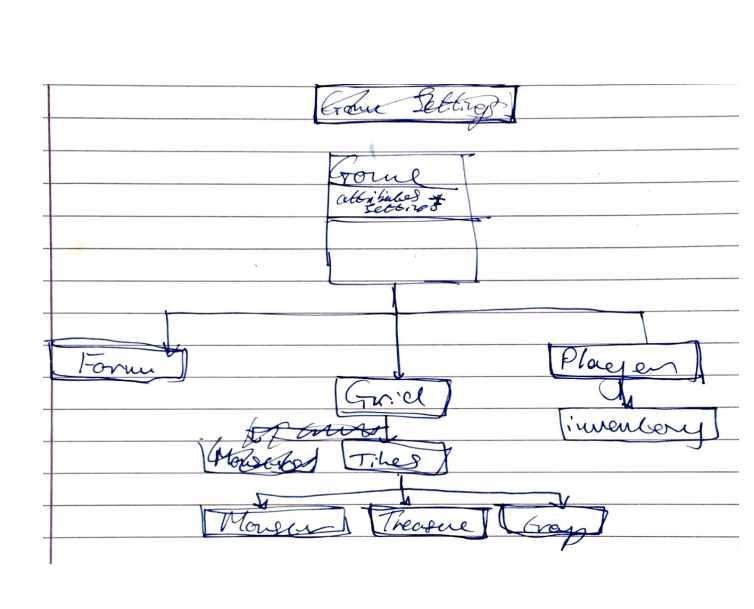
\includegraphics[width = 0.6\textwidth]{diagram_one}





































\end{document}